%%%%%%%%%%%%%%%%%%%%
% EVALUATION
%%%%%%%%%%%%%%%%%%%%
\section{Evaluation}
\label{sec:eval} 
%
In this section, we analyze the protection benefits and overheads
introduced by Harbor memory protection mechanisms.
%
We first present microbenchmarks that measure Harbor's CPU overhead
and resource utilization for a software-only implementation.
%
We follow that with a similar evaluation for UMPU.
%
Later, we compare the application level performance in the presence of
various protection mechanisms.
%
We conclude this section with a discussion on the various programming
errors that can be detected and prevented by Harbor memory protection.
%
%--------------------------------------------------------------
\subsection{Harbor CPU Overhead Microbenchmarks}
%
We first present microbenchmarks that measure Harbor's CPU overhead.
%
Overhead was measured using Avrora~\cite{titzer05avrora}, a cycle
accurate node and network simulator for the Mica family of sensor
nodes.
%
Measurements were averaged across multiple application scenarios.
%
%--------------------------------------------------------------
\subsubsection{Overhead of Harbor Primitives}
%
Table~\ref{tab:harbor_routines} summarizes the results for all of Harbor's
protection primitives.
%
All these routines are implemented in assembly for optimizing performance.
%
The registers used in these routines are saved to the run-time stack.
%
Many CPU cycles are spent in push and pop operations.
%
This overhead could be significantly reduced by dedicating one or more
registers for Harbor's exclusive use; the cross-compiler would be directed
to ignore these registers entirely.
%
%% The cross compiler can be directed to produce binary that does not use few registers.
%% %
%% The registers left unused by compiler can be used freely in memory protection assembly routines without saving them to stack.
%
However, \texttt{avr-gcc} does not have stable support for dedicated registers.
%

\begin{table}[htdp]
\centering
\small{
\begin{tabular}{|l|c|}
	\hline
	Function Name & Cost\\
	\hline
	\texttt{write\_access\_check} & 65~cyc\\
	\texttt{cross\_domain\_call} & 65~cyc\\
	\texttt{cross\_domain\_return} & 28~cyc\\
	\texttt{func\_entry\_stub} & 38~cyc\\
	\texttt{func\_exit\_stub} & 38~cyc\\
	\hline
\end{tabular}}
\caption{CPU Overhead of Memory Protection Routines}
\label{tab:harbor_routines}
\end{table}

Our implementation of some of the \texttt{cross\_domain\_call} and
\texttt{cross\_domain\_return} assumes that the modules follow the
\texttt{avr-gcc} ABI.
%
This optimizes the performance of these routines as they are free to use
the caller used registers defined in the ABI.
%
In addition, these routines can also use the scratch registers.
%
This results in a total of six registers that can be used by in the
AVR architecture (\texttt{R0, R1, R26, R7, R30 and R31}).
%
However, the implementation of the \texttt{function\_entry\_stub} and
\texttt{function\_exit\_stub} cannot use the caller-used registers
because some of the compiler inserted routines for integer arithmetic
do not follow the regular calling conventions.
%--------------------------------------------------------------
\subsubsection{Memory Map Overhead}
%
Overhead is also introduced during dynamic memory allocation, deallocation,
and transfer, since the memory map must be updated.
%
Table~\ref{tab:malloc_comparison} compares the overhead of memory
allocation routines in the presence and absence of the protection
mechanism.
%
The overhead depends upon the size of memory block that is being
allocated, freed or transferred.
%
The average size of the memory block used by all the three operations in
our experiments was 16 bytes.
%
The numbers in Table~\ref{tab:malloc_comparison} are an average
measurement of the execution time obtained from a long running
simulation of the Surge application~\cite{woo03surge}.
%
The relatively higher overhead of \verb+ker_change_own+ and \verb+ker_free+
calls is due to additional checks introduced to prevent illegal
ownership transfer or freeing of memory blocks by non-owners.
%
\begin{table}[htdp]
\centering
\small{
\begin{tabular}{|l|c|c|}
	\hline
	Function Name & Normal & Protected \\
	\hline
	\texttt{ker\char`\_malloc}  & 343~cyc & 610~cyc \\
	\texttt{ker\char`\_free} & 138~cyc & 425~cyc\\
	\texttt{ker\char`\_change\char`\_own} & \hphantom{0}55~cyc & 365~cyc \\
	\hline
\end{tabular}}
\caption{CPU Overhead for Dynamic Memory Calls}
\label{tab:malloc_comparison}
\end{table}
%
%--------------------------------------------------------------
\subsection{Harbor Resource Utilization Microbenchmarks}
%--------------------------------------------------------------
\subsubsection{Resource Utilization of Harbor Primitives}
%
Increases in code and data memory utilization due to Harbor's
protection mechanisms are shown in
Table~\ref{tab:kernel_size_comparison}.
%
Code memory usage increases by about 15\% in a protected kernel
relative to an unprotected kernel.
%
This increase is mainly due to the memory map and cross domain call
jump table mechanisms.
%
There is no significant change in program memory usage going from two
protection domains to multiple protection domains.
%
Data memory usage increases relative to an unprotected kernel by at
most 5\% and 9.5\% in 2-domain and 8-domain systems, respectively.
%
The main culprit is the memory map, which takes 128 and 256~bytes in 2-
and 8-domain systems.  (There are 28~additional bytes of constant
overhead.)
%
This is the maximum possible overhead, as this memory map configuration
stores layout and ownership information for the entire address space.
%
%% Memory map sizes are 128 bytes and 256 bytes respectively for
%% two-domain and multi-domain configurations.
%
By modifying data layout, the portion of address space that requires a
memory map can be reduced.
%
For example, in SOS, memory map is needed only for the heap and the safe
stack; by abutting these data structures, the memory map can be
reduced to 70 or 140~bytes for 2- and 8-domain protection, respectively.
%
%% By abutting these two data-structures, size of memory map required can be reduced to 70 bytes for two-domain protection (140 bytes for multi-domain protection)\footnote{There is 28 byte constant overhead. Therefore total overhead is 98 bytes}.
%
\begin{table}[htdp]
\centering
\small{\def\X{\hphantom{0}}
\begin{tabular}{|l|c|c|c|c|c|}
	\hline
	Memory & Raw & \multicolumn{2}{c|}{$\Delta$ (2 domains)} & \multicolumn{2}{c|}{$\Delta$ (8 domains)}
	\\
	\hline
	Flash\raise1pt\hbox{\strut}  & 41796 B & +6146 B & +14.7\% & +6228 B & +14.9\% \\
	RAM (Max) & \X{}2892 B & \X{}+148 B & \X{}+5.1\% & \X{}+276 B &
	\X{}+9.5\% \\
	RAM (Min) & \X{}2892 B & \X{}\X{}+98 B & \X{}+3.4\% & \X{}+168 B &
	\X{}+5.8\% \\
	\hline
\end{tabular}}
\caption{Code and Memory Overhead for Blank SOS Kernel for Mica2}
\label{tab:kernel_size_comparison}
\end{table}
%------------------------------------------------------------
\begin{table}[htdp]
\centering
\small{\def\X{\hphantom{0}}\def\XX{\X\X}
\begin{tabular}{|l|c|c|c|}
	\hline
	Module & Raw & \multicolumn{2}{c|}{$\Delta$ (2 or 8 domains)} \\
	\hline
	Blink\raise1pt\hbox{\strut} & \XX{}150 B & \XX{}+48 B & +32\%\\
		% 150B -> 198B
	Tree Routing & \X{}2820 B & +1658 B & +59\%\\
		% 2820B -> 4478B
	Surge & \XX{}542 B & \X{}+350 B & +65\%\\
		% 542B -> 892B
	Outlier Det. & \X{}1312 B & \X{}+738 B & +56\% \\
		% 1312B -> 2050B
	DVM & 13072 B & +6652 B & +51\%\\
		% 13072B -> 19724B
	FFT & \X{}3016 B & \X{}+894 B & +30\% \\
		% 3016B -> 3910B
	\hline
\end{tabular}}
\caption{Code Size Increase of Mica2 SOS Modules}
\label{tab:module_size_comparison}
\end{table}

\subsubsection{Size overhead of Sandboxing Modules}
%
Finally, we evaluate the relative increase in size of modules due to
introduction of checks by the binary rewriter.
%
As noted in Table~\ref{tab:module_size_comparison}, there is a significant
increase in the relative code size of sandboxed binaries as compared to raw
binaries.
%
This is mainly caused due rewriting all store instructions to a long
sequence of instructions that call the memory map checker
(Figure~\ref{fig:inlinechecks}).
% 
This overhead could be significantly reduced by using dedicated registers
to eliminate all push/pop instructions in the sequence, and/or by adding
static analysis to eliminate some redundant checks.
%
%
%---------------------------------------------------------------------------
\subsection{UMPU CPU Overhead Microbenchmarks}
%
In this section, we evaluate the CPU overhead of UMPU primitives.
%
We have implemented the hardware components of UMPU by extending
the architecture of the AVR ATMEGA103
microcontroller~\cite{avr103manual}~\cite{avropencores}.
%
The VHDL model of the processor is fully synthesizable.
%
We have instantiated the processor on Xilinx Vertex 2 Pro XC2VP30 FPGA.
%
Our performance overheads are measured using Modelsim 6.0
simulator~\cite{modelsim}.
%
The software library and applications were compiled using
\texttt{avr-gcc} cross compiler.
%
Table~\ref{tab:umpumicrobmperf} contains the CPU overhead of the UMPU
primitives.
%
A comparison to Harbor's software based implementation
(Table~\ref{tab:harbor_routines}) clearly indicates the superior
run-time performance of the primitives implemented in hardware.
%
\begin{table}[htdp]
\centering
\small{
\begin{tabular}{|l|l|c|}
	\hline
	UMPU Function Unit & Function Name & Cost\\
	\hline
	Memory Map Controller &\texttt{write\_access\_check} & 1~cyc\\
	Cross Domain Call Unit &\texttt{cross\_domain\_call} & 5~cyc\\
	Cross Domain Ret. Unit &\texttt{cross\_domain\_return} & 5~cyc\\
	Safe Stack Unit &\texttt{func\_entry\_stub} & 0~cyc\\
	Safe Stack Unit &\texttt{func\_exit\_stub} & 0~cyc\\
	\hline
\end{tabular}}
\caption{Overhead of UMPU Primitives}
\label{tab:umpumicrobmperf}
\end{table}
%

The \texttt{write\_access\_check} implemented by the memory map
controller requires one clock cycle to read the appropriate memory map
byte from RAM.
%
The address translation operation and the permission checking is
implemented by combinational logic units that do not introduce any overhead.
%

Cross domain call and return have an overhead of five clock cycles
when implemented in hardware.
%
The overhead occurs because the current domain identity, stack bound
and return address have to be pushed to the safe stack before they can
be updated with new values.
%
The total information that needs to be pushed to the stack is five
bytes and only one byte can be written every clock cycle.
%
Similarly on the cross domain return, the five clock cycles are
expended in restoring the values read from the safe stack.

Saving and restoring return addresses to the safe stack does not
introduce any added overhead.
%
This is because the hardware unit for safe stack simply takes over the
address bus when the processor is pushing the return address to the
run-time stack.
%
By stealing the address bus from the processor, the hardware unit is
able to simply redirect the store of the return addresses to the safe
stack.

The memory map software library in UMPU is identical in functionality
and implementation to the Harbor memory map API.
%
Therefore, the CPU overhead of the memory management functions (\texttt{malloc},
\texttt{free} and \texttt{change\_own}) is same as the corresponding
Harbor's functions (Table~\ref{tab:malloc_comparison}).
%
%---------------------------------------------------------------------------
\subsection{UMPU Resource Utilization}
%
The UMPU resource utilization comprises of the increased gate count
due to the hardware extensions and the FLASH and RAM utilization of
the software library.
%
In this section, we are primarily concerned only with the gate count
and area.
%
The FLASH and RAM utilization of the software library in UMPU is
similar to Harbor (Table~\ref{tab:kernel_size_comparison}).



%
We measured the gate count of the UMPU components using the Xilinx ISE
8.2i~\cite{xilinxlink} design and synthesis tools.
%
Table~\ref{tab:umpuarea} summarizes the area overhead of UMPU extensions.
% 
\begin{table}[htdp]
\centering
\small{\def\X{\hphantom{0}}\def\XX{\X\X}\def\XXX{\XX\X}\def\Y{\raise1pt\hbox{\strut}}
\begin{tabular}{|l|c|c|c|c|}
	\hline
	Component & Raw & \multicolumn{2}{c|}{$\Delta$ (2 or 8 domains)} & Fraction \\
	\hline
	AVR Core   & \XX{}16419 Gates &   +10504 Gates & +64.00\% &\XX{}0.4\%\\
	Data Mem.  & \X{}131099 Gates & \XXX{}+0 Gates &  +0.00\% &\XX{}3.0\%\\
        Prog Mem.  &    4195531 Gates & \XXX{}+0 Gates &  +0.00\% & \X{}96.5\%\\
        AVR Total  &    4349691 Gates &   +10504 Gates &  +0.24\% &   100.0\%\\   
	\hline
\end{tabular}}
\caption{Area Increase of UMPU}
\label{tab:umpuarea}
\end{table}

The area of the chip is measured in terms of the number of equivalent
logical gates.
%
The UMPU components residing within the core of the chip increase its
area by 64\%.
%
However, the core occupies only 0.4\% of the total chip area; a very
small fraction.
%
Therefore, the total increase in the area of the chip is only 0.24\%.
%
The Xilinx Vertex FPGA used to synthesize the processor does not have
Flash memory which is typically used to implement program memory.
%
Therefore, the program memory mapped to SRAM block cells occupies a
disproportionately large fraction (96.5\%) of the overall chip area.
%

We estimate the increase in the fraction of area occupied by the CPU
core in a typical sensor node processor after the introduction of the
protection mechanisms.
%
The Spec node~\cite{jasonhillthesis}, is a single chip implementation
of a sensor node comprising of a RISC CPU core, SRAM, 900 MHz RF
Transceiver, collection of communication hardware accelerators and an
analog-digital converter.
%
The RISC CPU core used in Spec is similar to the AVR core comprising
of 8-bit datapath and 16-bit instructions.
%
It also has 32 8-bit general purpose registers.
%
The area of the CPU core and ALU in Spec is 0.3920 mm$^2$.
%
Incorporating the UMPU extensions would increase this area by 0.2501
mm$^2$ to 0.6429 mm$^2$ (assuming an identical area overhead of 64\%).
%
The total die area of the Spec node is 6.25 mm$^2$.
%
Therefore, the fraction of die area occupied by the CPU core will
increase from 6.27\% to 10.28\% in the Spec node equipped with UMPU
extensions (Figure~\ref{fig:dieareacmp}).
%
This is a negligible increase in the fraction of area occupied.
%
The packing efficiency of logic in a chip is never 100\%.
%
Therefore, the UMPU extensions can be accommodated without any increase
to the chip die area.
%
\begin{figure}[htbp]
  \centering
   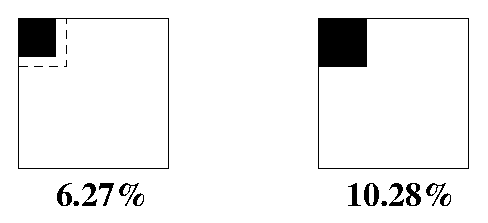
\includegraphics[height = 1.15in, keepaspectratio=true]{figures/areacomp.eps} 
   \caption{Area overhead comparison}
   \label{fig:dieareacmp}
\end{figure}

%
We next measure the fraction of the total increase in the gate count
due to the various UMPU components (Table~\ref{tab:umpuareacomp}).
%
\begin{table}[htdp]
\centering
\tiny{\def\X{\hphantom{0}}\def\XX{\X\X}\def\XXX{\XX\X}\def\Y{\raise1pt\hbox{\strut}}
\begin{tabular}{|l|c|c|}
	\hline
        \hline
	\textbf{Function Unit} & \textbf{Area} & \textbf{Fraction}\\
	\hline
        \hline
        Fetch Decoder Modifications & \XX{}272~Gates & \XX{}2.6\%\\
        \hline
	Memory Map Controller Config. & \XX{}870~Gates & \XX{}8.3\%\\
        \hline
        Memory Map Addr. Trans.       & \XX{}687~Gates & \XX{}6.5\%\\
        \hline
        Memory Map Perms Checker & \XX{}783~Gates& \XX{}7.5\%\\
        Run-Time Stack Checker & & \\
        \hline
        Safe Stack & \X{}2188~Gates & \X{}20.8\%\\
        Cross Domain Call \& Ret State m/c & &\\
	\hline
        Domain Tracker & \X{}1363~Gates & \X{}13.0\%\\
        Cross Domain Call Trig. &&\\
        \hline
        Domain Bounds Checker & \X{}3160~Gates & \X{}30.0\%\\
        \hline
        Exception Generator & \XXX{}31~Gates & \XX{}0.3\%\\
        \hline
        Ram Bus Arbiter & \XX{}390~Gates & \XX{}3.7\%\\
        \hline
        Interrupt Controller Modifications & \XX{}760~Gates & \XX{}7.2\%\\
        \hline
        \hline
        \textbf{Total} & \textbf{10504~Gates} & \textbf{100\%}\\
        \hline
        \hline
\end{tabular}}
\caption{Area breakup of UMPU extensions}
\label{tab:umpuareacomp}
\end{table}

%
The maximum increase in the area occurs due to the Domain Bounds
Checker.
%
We store the domain bounds in a register file to improve the
performance of UMPU during cross domain calls and returns.
%
If area is a primary concern, then the domain bounds can be stored in
a look-up table within RAM or FLASH (Section~\ref{sec:dombndschecker})
%
%--------------------------------------------------------------------------
\subsection{Relative Application Performance}
%
In this section, we measure Harbor performance impact on
applications.
%
We also compare the performance of the software only implementation of
protection with the hardware accelerated UMPU extensions.
%
%----------------------------------------
\subsubsection{Fast Fourier Transform}
%
Many sensor network applications are heavily duty-cycled and therefore
not CPU intensive.
%
However, some are not~\cite{ben06vango}, and for our first benchmark,
we choose a CPU intensive Fast Fourier Transform (FFT).  
%
This should present a realistic idea of Harbor's
costs for challenging applications.
%
The FFT module receives a buffer of 64 samples represented as 16-bit
fixed-point integers (we do not measure the cycles required to obtain the
samples).
%
It transforms the samples in place and outputs results to the same buffer.
%
As shown in Table~\ref{tab:perf_comp}, FFT running on ATMEGA128 (Mica2
sensor node) takes 3.63~ms to execute in normal mode and 17.28~ms in the
protected mode.
%
This gives Harbor a slowdown factor of 4.76.
%
FFT running ATMEGA103 takes 8.24~ms to execute.
%
The execution time of FFT on ATMEGA103 is about two times slower than
on ATMEGA128.
%
This is primarily due to enhanced instruction set of ATMEGA128 which
in particular supports hardware accelerated 8 bit multiplication.
%
FFT routine contains a lot of multiplication operations.
%
The execution of FFT with UMPU protection takes 8.41~ms; a slowdown
factor of only 1.02.
%
In other words, the relative overhead of a computationally intensive
FFT operation with UMPU is only 2\%.
%
%----------------------------------------
\subsubsection{Outlier Detector}
The next experiment is another challenging application, an outlier detector.
%
The outlier detector samples a set of sensor values and stores them in a buffer.
%
Once the buffer is filled, it computes the distance between all pairs of samples in the buffer and stores the result in a matrix.
%
Using a distance threshold, the algorithm marks the distance measurements in the matrix that are greater than the threshold.
%
If the majority of the distance measurements for a sensor readings are marked, then the sensor reading is classified as an outlier.
% %%% <------------- Need Reference !!
%This algorithm is currently being used in the Rate-Adaptive Time Synchronization system.
%
This application is memory write intensive and the matrix operations are easily prone to buffer overflow errors.
%

\begin{table}[htdp]
\centering
\small{\def\X{\hphantom{0}}\def\XX{\X\X}\def\XXX{\XX\X}\def\Y{\raise1pt\hbox{\strut}}
\begin{tabular}{|l|c|c|}
	\hline
	Module & Time (ms) & Slowdown\\
	\hline
	FFT-ATMEGA128\Y		& \XX{}3.63\X & --- \\
        FFT-ATMEGA103\Y         & \XX{}8.24\X & --- \\
        FFT-UMPU                & \XX{}8.41\X & \XXX{}1.02 \\
	FFT-Harbor		& \X{}17.28\X & \XXX{}4.76 \\
	\hline
	Outlier-ATMEGA128\Y	& \XX{}0.18\X & --- \\
        Outlier-ATMEGA103\Y     & \XX{}0.34\X & --- \\
        Outlier-UMPU            & \XX{}0.36\X & \XXX{}1.06\\
	Outlier-Harbor		& \XX{}1.47\X & \XXX{}7.94 \\
	Outlier-DVM		& 102.47\X & \X{}554.50 \\
	Outlier-DVM-Harbor	& 268.32\X & 1452.72 \\
	\hline
	\multicolumn{2}{|l|}{Sort with Mat\'e VM script~\cite{asvm05nsdi}\Y} & \X{}115\hphantom{.0} \\
	\hline
\end{tabular}
}
\caption{Relative Performance of Applications}
\label{tab:perf_comp}
\end{table}

We consider three systems that can protect against such errors,
%
Harbor, UMPU and the Dynamic Virtual Machine (DVM)~\cite{balani06dvm}, an extensible
domain-specific interpreter that performs a bounds check on every write.
%
DVM's bounds checks are in some ways more stringent than Harbor's
protection, since they also prevent scripts from corrupting \emph{their
own} memory.  However, errors in DVM's native code implementation might
corrupt any memory on the node.
%
We implemented the outlier detector as a DVM script that is interpreted on
sensor sampling timer events.
%
The execution time of the script was measured to be 102.9~ms.
%
However, some of this time is also spent within the kernel to actually sample the sensor data.
%
The sampling time was measured to be 0.49~ms, so
%
the script's true execution time is 102.41~ms.
%
This is over 500 times longer than an outlier detector implemented as a raw
binary, as Table~\ref{tab:perf_comp} shows.
%
The high overhead is due to DVM interpretation.
%
The outlier detector script uses many low-level operations.
%
Prior work has shown that this kind of script has high overhead; for
example, a Mat\'e script that sorts an array using low-level
operations takes 115~times longer than a script that sorts an array
with a single ``sort'' operation~\cite{asvm05nsdi}.
%
While DVM's overhead could be reduced by adding high-level
instructions that perform complex operations in native code, these
high-level instructions might themselves contain bugs.
%
Harbor's protection is much less expensive than interpretation overhead.
%
Sandboxing slows down the native code implementation by a factor of 7.94.
%
Perhaps more surprising, sandboxing DVM slows it down only by an
additional factor of 2.6.
%
%% DVM can thus benefit from Harbor's domain-level protection by installing high level instruction set extensions in separate domains.
%
Here, DVM provides fine grained protection (at the level of individual
memory objects) to scripts and Harbor provides coarse grained protection
(at the level of domains) to the system running DVM.
%
Finally, we evaluate the performance of the outlier detector with
UMPU.
%
As shown in Table~\ref{tab:perf_comp}, the hardware accelerated
protection of UMPU causes a slowdown of only 1.06; the relative
execution overhead is only 6\%.
%
UMPU provides all the protection benefits of Harbor with a very low
performance impact.
%
%% DVM protects against more faults than Harbor, since it bounds 
%
%
%% Next, we measure the execution time of running the outlier detector as a script within a sandboxed DVM.
%% %
%% This experiment measures the relative slowdown in the execution of the DVM after it has been sandboxed.
%% %
%% As can been seen from the Table~\ref{tab:perf_comp}, the extra
%% protection introduced by Harbor slows down the execution of the DVM by
%% a factor of 2.6.

%----------------------------------------
\subsubsection{Buffer Writer}
%
A final challenging, write-intensive application is a simple buffer writer, which
%
allocates a memory block and completely fills its
contents with arbitrary data.
%
This application simulates a very common behavior of sensor network
applications, namely copying sampled sensor data into a buffer that can be
transmitted into the network.
%
A common programming mistake in such applications is to overflow the
buffer.
%
%We consider two systems that protect against such buffer overflow errors.
%
%First, Dynamic Virtual Machine(DVM)~\cite{balani06dvm}, an extensible domain specific interpreter that performs bounds check on every write operation to buffer.
%
%Second, SOS kernel with multi-domain protection (Harbor) that uses memory map checker to prevent buffer overflow.
%
Figure~\ref{fig:buff_writer} plots execution time of the buffer writer on
DVM, Harbor, and native SOS for varying buffer sizes.
%
The average slowdown factor of Harbor relative to native SOS for this
application was 13.3.
%
%% The application is very write-intensive and represents a worst-case
%% workload for Harbor.
%
The average slowdown factor of DVM relative to native SOS was about 1200.
%
%% The fine-grained bounds check performed by DVM for a write operation is
%% more expensive than the memory map checks done by Harbor.
%
UMPU had an average slowdown of only 1.16.

%From the plot, we can clearly conclude that sandboxing overhead is significantly lower than interpretation overhead of DVM.
%
%Interpretation overhead of DVM is reduced by adding high level instructions that perform complex operations.
%
%Instructions implemented in native code are not type safe.
%
%DVM can benefit from Harbor's domain-level protection by installing high level instruction set extensions in separate domains.
%
%Thus, DVM provides fine grained protection (at the level of individual memory objects) to scripts and Harbor provides coarse grained protection (at the level of domains) to instruction set implementation.
%
%Together, application execution is guaranteed to be memory safe.
%
%
%We also compare execution time of Buffer Writer on native SOS kernel and protected SOS kernel.
%
%It is evident that memory protection benefits come with a performance cost.
%
%Suitability of memory protection is dependent upon performance requirements of application.
%
%CPU bound applications will not benefit much from software based memory protection techniques.
%
%However, most sensor network applications have a very low CPU utilization~\cite{tkernel06sensys}.

\begin{figure}[htpb]
 \centering
  \mbox{
    \subfigure[Harbor Overhead]{\label{fig:buffwrharbor}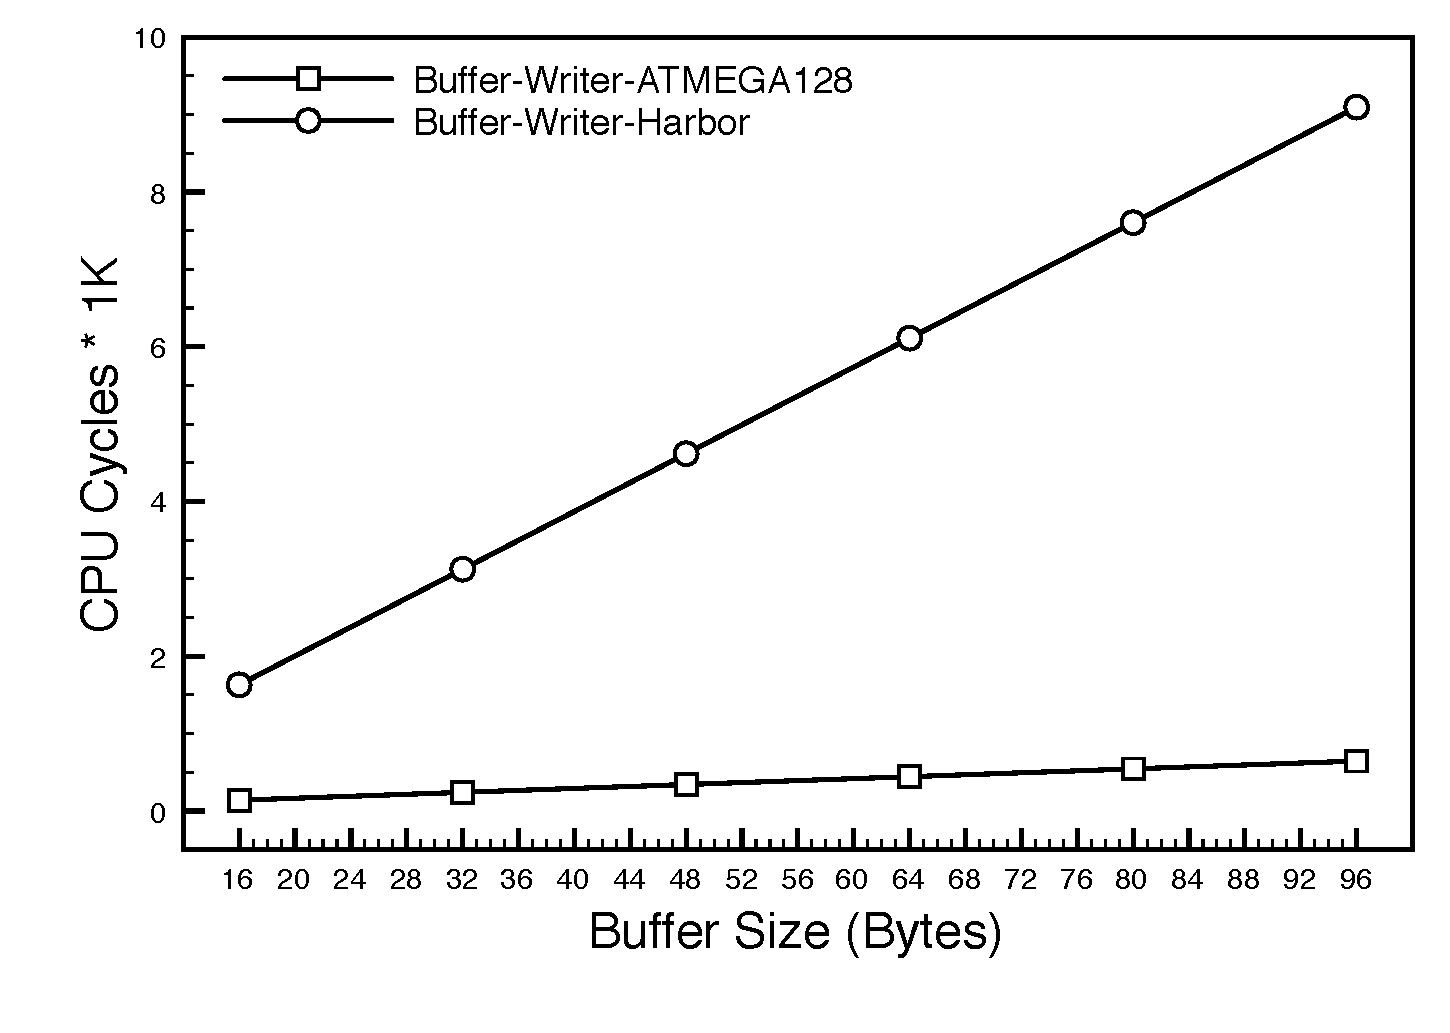
\includegraphics[width=1.8in,
      keepaspectratio = true]{figures/bufferwriterharbor.eps}}
    \hspace{0.05in}
    \subfigure[DVM Overhead]{\label{fig:bffwrdvm}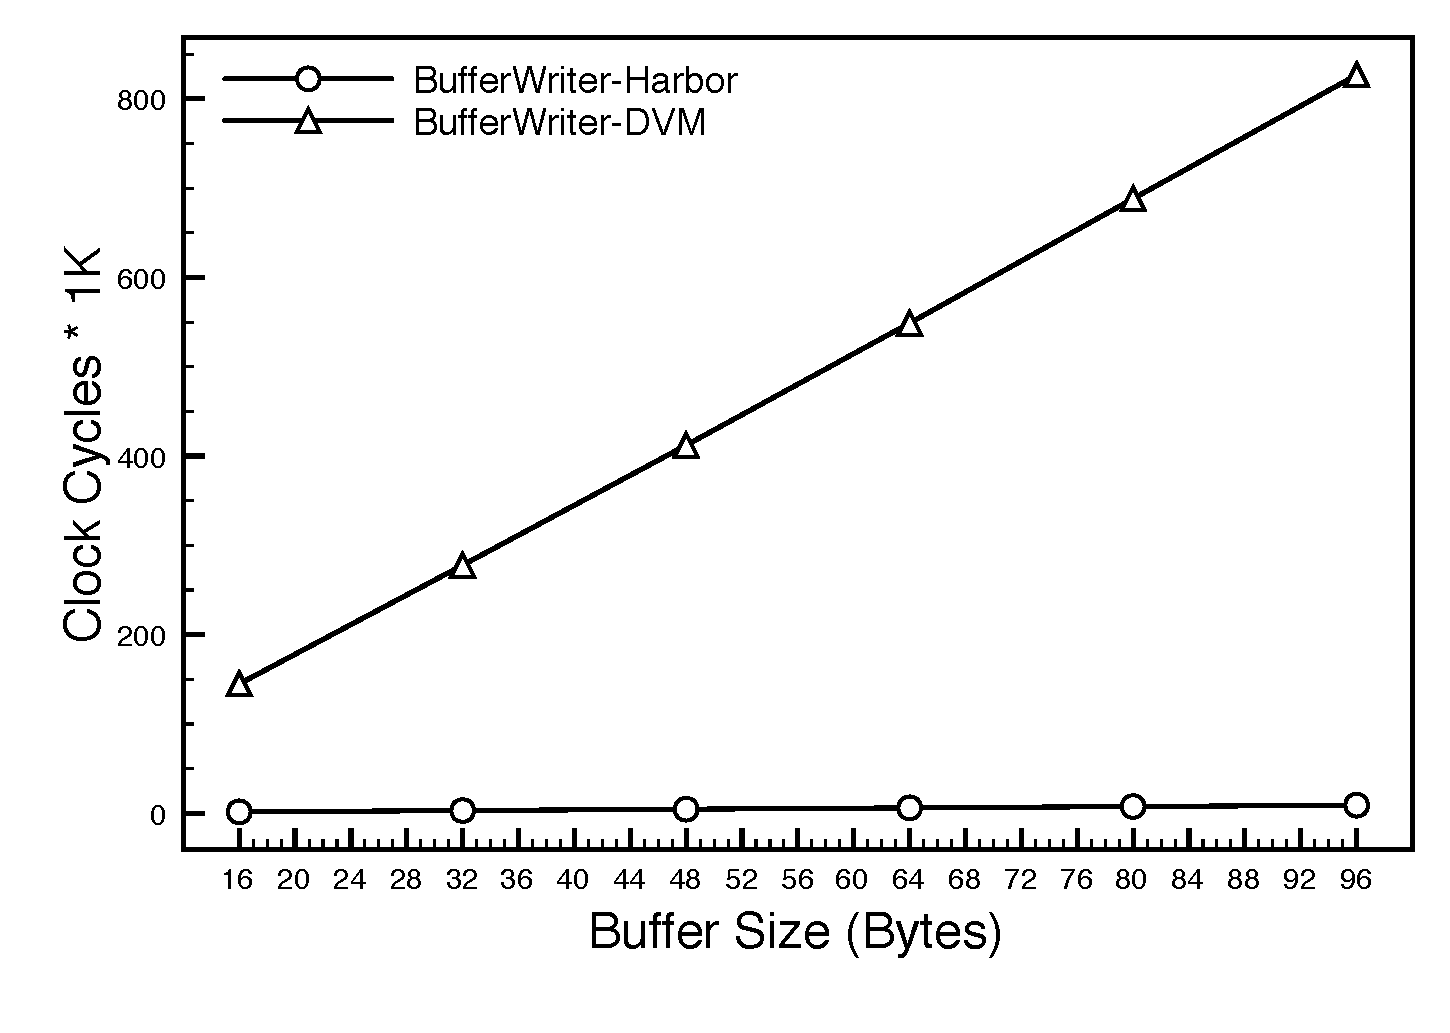
\includegraphics[width=1.8in,
      keepaspectratio = true]{figures/bufferwriterdvm.eps}}
    \hspace{0.05in}
    \subfigure[UMPU Overhead]{\label{fig:bffwrumpu}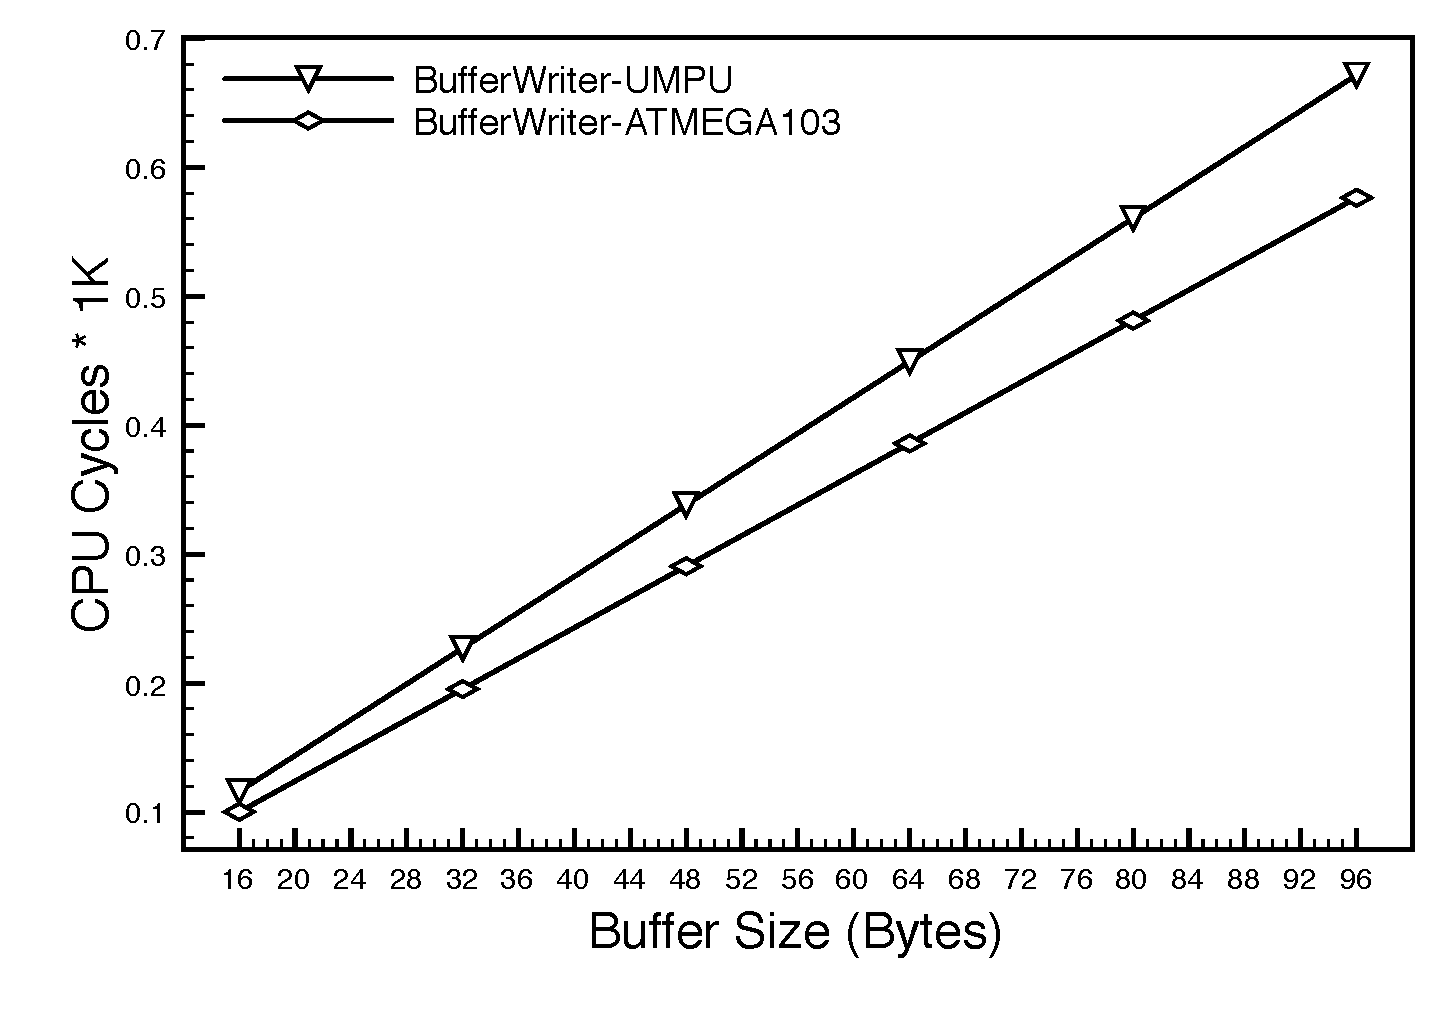
\includegraphics[width=1.8in,
      keepaspectratio = true]{figures/bufferwriterumpu.eps}}
  }
  \label{fig:buff_writer}
  \caption{Buffer Writer Performance}
\end{figure}   

%----------------------------------------
\subsubsection{Data Collector}
%
We next consider a typical duty-cycled sensor network application,
namely data gathering through a collection tree.
%
Our experiment setup was a simulated network of 5 Mica2 motes arranged
in a linear topology to form a two-hop network to a base station.
%
All nodes were installed with an SOS kernel with 8-domain Harbor protection.
%
When the network was up, the two-module data collection application was
installed on all nodes.
%
First, a tree building and maintenance module~\cite{woo03surge} was
distributed; then
%
the Surge module, which periodically samples light sensor data and sends it
to the base station via the collection tree, was installed.
%
The two modules were installed in different protection domains.
%
Harbor's impact on the complete application was measured by profiling CPU
active time in the Avrora simulator.
%
CPU active time was observed to be 8.41\% and 8.56\% over a duration
of 30 minutes for normal and protected mode operation, respectively. 
%
The relative increase in CPU utilization for a protected system is
thus only 1.85\% compared to an unprotected system.
%
In most sensor network applications, absolute CPU utilization is even
lower~\cite{tkernel06sensys}.
%
The increased overhead is a small price to pay for the improved
reliability provided by the software-based memory protection.
%----------------------------------------
\subsubsection{SOS Serial Stack}
%
Sensor network software needs to respond to events occurring in the
physical environment.
%
Efficient interrupt handling is critical to ensure a reactive system.
%
In this subsection, we evaluate the performance impact of memory
protection on the serial driver's interrupt service routine.
%
We isolate the Serial Stack from the SOS kernel and install it in a
separate protection domain.
%
The Serial Stack in SOS is a complex system comprising of multiple
layers (shown in Figure~\ref{fig:serialstack}) that implements the
High-Level Data Link Control (HDLC) protocol for communication between
a pair of nodes.
%
\begin{figure}[htbp]
  \centering
   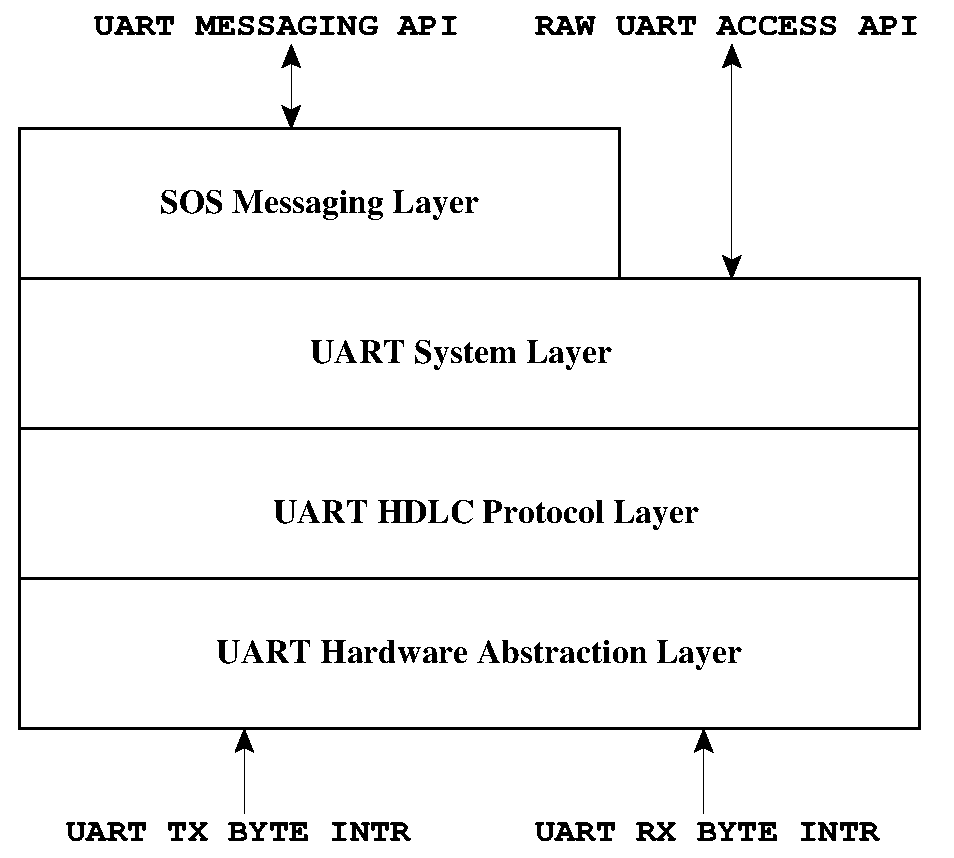
\includegraphics[height = 1.5in,
   keepaspectratio=true]{figures/serialstack.eps} 
   \caption{SOS Serial Stack Layers}
   \label{fig:serialstack}
\end{figure}
%

Our experiment set up consists of a sensor node simulated in Modelsim
with UMPU enabled.
%
An application periodically sends a SOS message outside the
sensor node through the serial port.
%
The transmitted message is echoed back to the sensor node and is
received by the application.
%
The UART hardware and the serial stack is capable of full-duplex
operation.
%
All the processing in the serial stack occurs within the send and
receive interrupts.
%
%
\begin{figure}[htpb]
  \label{fig:intrtrace}
  \centering
  \mbox{
    \subfigure[Rx Interrupt Latency]{\label{fig:rxintr}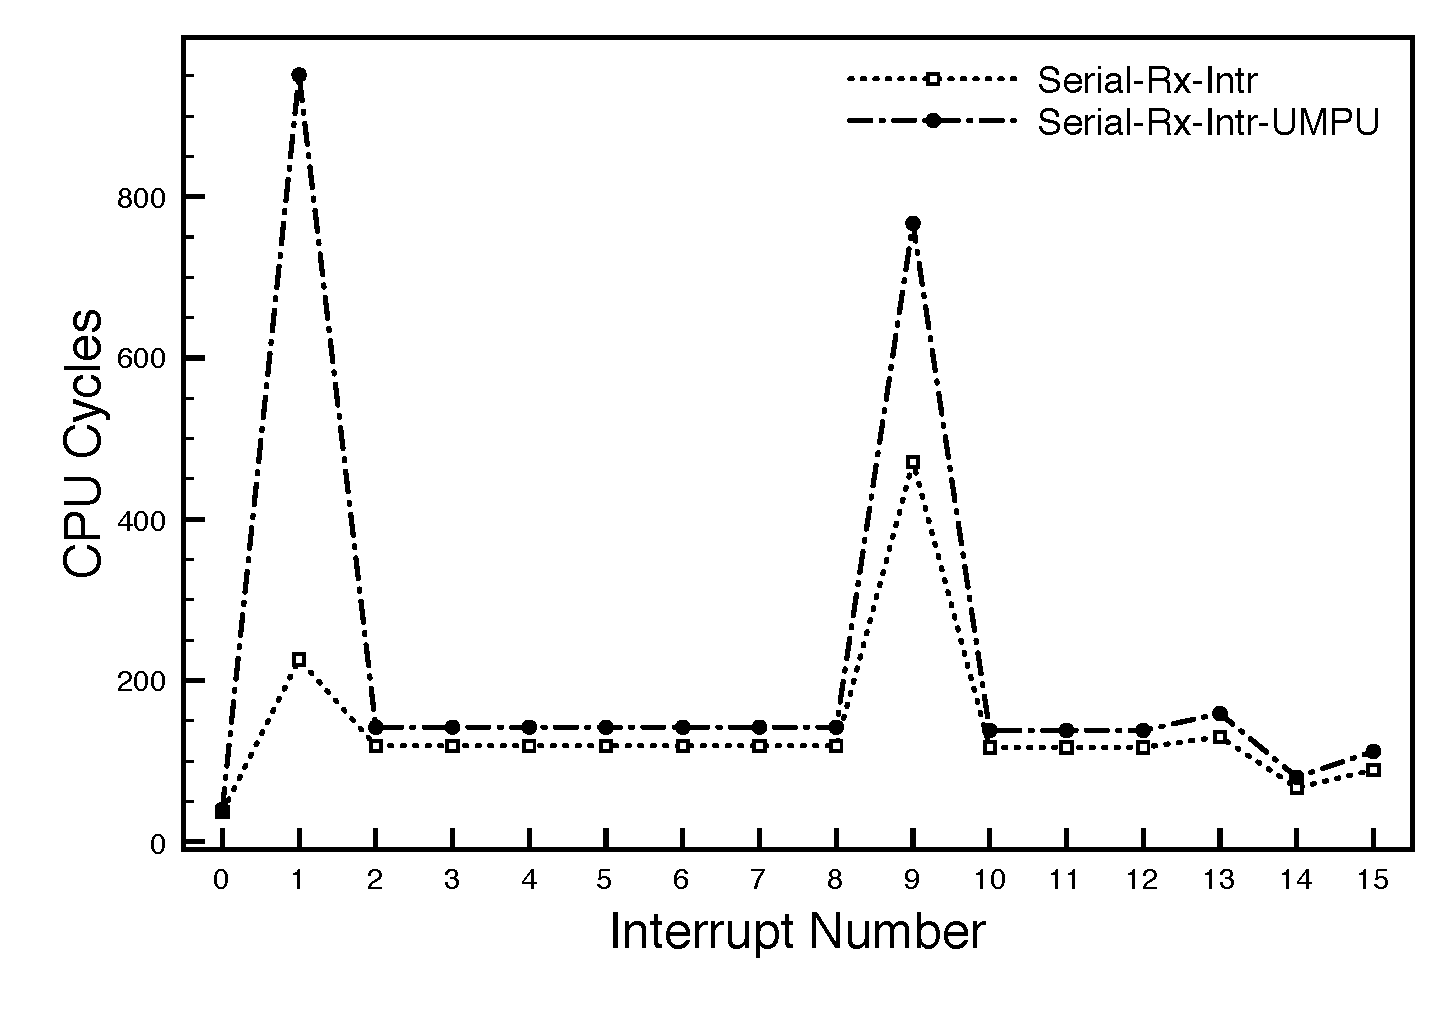
\includegraphics[width=2.5in,
      keepaspectratio = true]{figures/rxintr.eps}}
    \hspace{0.2in}
    \subfigure[Tx Interrupt Latency]{\label{fig:txintr}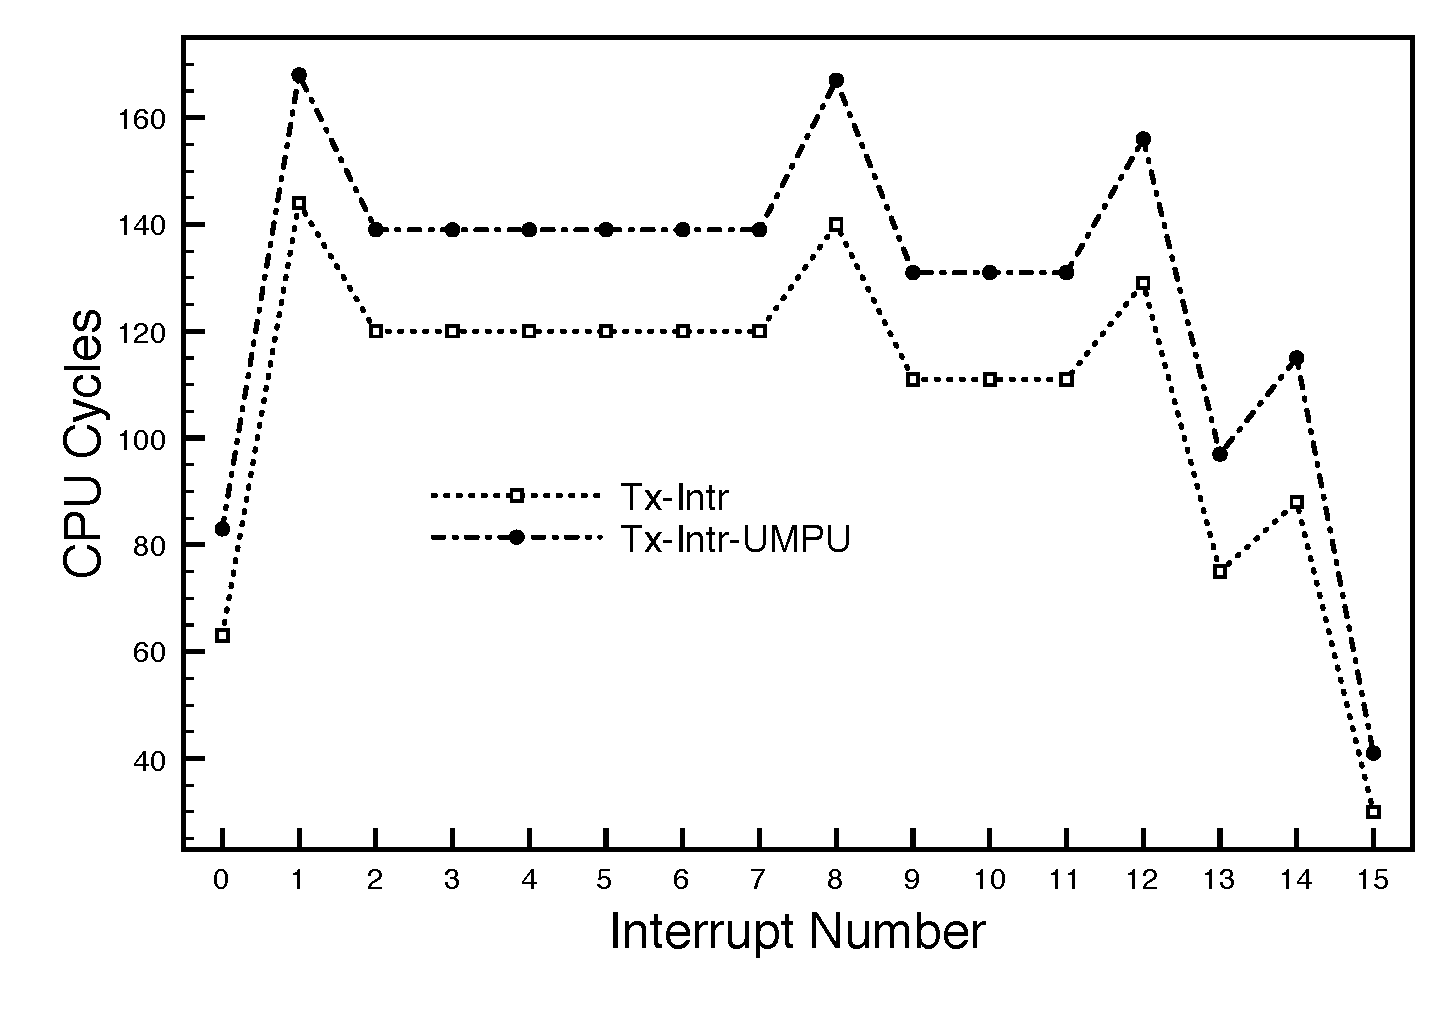
\includegraphics[width=2.5in,
      keepaspectratio = true]{figures/txintr.eps}}
  }
  \caption{Serial Stack Execution Trace}
\end{figure}   
%

Figure~\ref{fig:rxintr} contains a trace of the receive interrupt
service time with the protection enabled and disabled.
%
The execution time with UMPU enabled has a constant overhead of 23 clock
cycles except for interrupt number 1 and 9.
%
In the current UMPU implementation, all the interrupts originate in
the trusted domain and the control is transferred to the real
interrupt handler through a cross domain call.
%
The cross domain call through the jump table takes 13 clock cycles,
the corresponding cross domain return takes 9 clock cycles and the
execution of the interrupt handler takes one extra clock cycle to
check the memory map before storing the received byte.
%

Interrupt 1 allocates a SOS message data structure to store the
received message.
%
The UMPU disabled serial driver implementation allocates the message
from a pre-allocated pool of messages.
%
However, the UMPU enabled serial driver implementation cannot
pre-allocate a message pool as the memory map cannot track ownership
of data structures within an allocated segment.
%
This is a limitation of the memory map design.
%
Therefore, UMPU enabled serial driver has to incur the significantly
higher cost of memory allocation.
%

Interrupt 9 allocates the payload for the received message.
%
The higher latency of the UMPU enabled serial driver is due to the
higher overhead of memory allocation routines in the UMPU software
library.
%

The trace of the Transmit interrupt service time (Figure~\ref{fig:txintr}) shows only a constant
overhead caused due to the cross domain call mechanisms.
%
This experiment demonstrates that the protection benefits of UMPU can
be obtained without any loss in the performance of latency sensitive
routines.
%
%================================================================
% RESILIENCE TO APPLICATION FAULTS
%================================================================
\subsection{Experience} 
%
Harbor has been in use in SOS for several months, and has
%
discovered two memory corruption faults in application modules that had
been in active use for several months previously.
%
The first error was discovered while executing the data collection
application on a SOS kernel with 2-domain Harbor protection.
%
A programming error in the Surge module triggered an invalid memory access exception.
%
Figure~\ref{fig:surge_error} demonstrates the error.

\begin{figure} [h]
  \centering
\begin{small}
\begin{verbatim}
     // Size of routing header
     hdr_size = SOS_CALL(s->get_hdr_size, proto);
     // Using return value without checking 
     s->smsg = (SurgeMsg*)(pkt + hdr_size); 
     // Memory Corruption
     s->smsg->type = SURGE_TYPE_SENSORREADING;  
\end{verbatim} 
\vskip-\baselineskip
\end{small}
  \caption{Programming error in Surge module}
  \label{fig:surge_error}
\end{figure}

\noindent
%
The Surge module invokes a dynamic function call~\cite{ram05sos} to
the tree routing module to determine the size of the routing header.
%
Dynamic function calls are linked at run time, and fail with an error
code if the function provider is absent.
%
The code above fails to check whether \verb+hdr_size+ is an error code.
%
Nodes where the Surge module was installed before the tree routing module
would use an negative value for the routing header size and thereby corrupt
memory---specifically, heap metadata, which effectively resides in the
kernel domain.
%
Harbor detected this error and killed the offending application.


%
A second programming error was discovered in the tree routing module with
8-domain protection.
%
There were three active domains in the system: the kernel, the tree routing
module, and the buffer writer module.
%
The SOS kernel tracks the ownership of a message payload as it is passed from a source module to its destination module.
%
If the source module wishes to relinquish ownership, it sets a release flag while posting the message.
%
A destination module that wishes to write into the message payload is
\emph{required} to gain ownership through a \verb+sys_msg_take_data+ system
call.  If the source module set the release flag, this system call is
effectively a no-op.  If the source module did not set the flag, however,
then the system call makes a private copy of the payload owned by the
destination module.
%
Failure to call \verb+sys_msg_take_data+ could corrupt the source module's
memory.
%
The buffer writer module was not releasing the buffer, but the tree routing
module was not calling \verb+sys_msg_take_data+.
%
Harbor discovered this error when the tree routing module tried to
overwrite the message payload.
%

The errors described in this section occur under rare conditions and
are hard to detect during software testing.
%
However, the impact of these errors could be severe.
%
A system that can guarantee memory protection is indispensable for
building robust embedded software.






















